\documentclass[12pt,a4paper]{report}

% Packages
\usepackage[utf8]{inputenc}
\usepackage[T1]{fontenc}
\usepackage{amsmath}
\usepackage{amssymb}
\usepackage[lining]{ebgaramond}
\usepackage[cmintegrals,cmbraces]{newtxmath}
\usepackage{microtype}
\usepackage{geometry}
\usepackage{graphicx}
\usepackage{booktabs}
\usepackage{array}
\usepackage{xcolor}
\usepackage{hyperref}
\usepackage{float}
\usepackage{caption}
\usepackage{etoolbox}
\usepackage{enumitem}
\usepackage{makecell}
\usepackage{subcaption}
\graphicspath{{./fig/}}

% Page layout
\geometry{
    left=1.8cm,
    right=1.8cm,
    top=2.2cm,
    bottom=2.2cm
}

% Color definitions
\definecolor{crimson}{RGB}{153, 0, 0}

% Hyperlink settings
\hypersetup{
    colorlinks=true,
    linkcolor=crimson,
    urlcolor=crimson,
    citecolor=crimson
}

\tolerance=2000
\emergencystretch=2em

% Chapter/section title formatting
\usepackage{titlesec}
\titleformat{\chapter}{\normalfont\huge\bfseries}{}{0pt}{}[\vspace{0.3em}]
\titlespacing*{\chapter}{0pt}{0pt}{14pt}
\titleformat{\section}{\normalfont\Large\bfseries}{\thesection}{1em}{}
\titleformat{\subsection}{\normalfont\large\bfseries}{\thesubsection}{1em}{}

\setlength{\parindent}{0pt}
\setlength{\parskip}{4pt}

% Float spacing
\setlength{\floatsep}{6pt plus 2pt minus 2pt}
\setlength{\textfloatsep}{10pt plus 2pt minus 2pt}
\setlength{\intextsep}{10pt plus 2pt minus 2pt}
\setlength{\abovecaptionskip}{4pt}
\setlength{\belowcaptionskip}{0pt}
\captionsetup[figure]{skip=5pt, belowskip=2pt}
\captionsetup[table]{skip=2pt}
\BeforeBeginEnvironment{figure}{\vspace{4pt}}
\AfterEndEnvironment{figure}{\vspace{2pt}}
\AfterEndEnvironment{table}{\vspace{-6pt}}

% Question box: \question{text}
\newcommand{\question}[1]{%
    \hrule
    \vspace{0.2cm}
    #1
    \vspace{0.2cm}
    \hrule
    \vspace{0.5cm}
}

\begin{document}

\pagestyle{plain}

% ─────────────────────────────────────────────
%  Cover Page
% ─────────────────────────────────────────────
\begin{titlepage}
\centering
\vspace*{3cm}

{\fontsize{28}{34}\selectfont\bfseries Digital Communication IC Design\par}
\vspace{0.6em}
{\fontsize{20}{26}\selectfont\bfseries Homework 4\par}

\vspace{1.5cm}
\textcolor{crimson}{\rule{0.6\linewidth}{1.2pt}}
\vspace{1.5cm}

{\large\bfseries Student ID}\par
\vspace{0.4em}
{\large M11407439}\par

\vspace{0.8em}

{\large\bfseries Name}\par
\vspace{0.4em}
{\large MING-HONG, LIN}\par

\vspace{2cm}

{\large\bfseries Development Environment}\par
\vspace{0.8em}
\begin{tabular}{rl}
    \textbf{Language} & MATLAB R2025b, SystemVerilog \\[4pt]
    \textbf{Simulator} & Synopsys VCS S-2021.09, Verdi T-2022.06 \\[4pt]
    \textbf{AI Tool}  & Claude Opus 5.5 \\
\end{tabular}

\vfill

\textcolor{crimson}{\rule{0.6\linewidth}{0.6pt}}\par
\vspace{0.5em}
{\small Due Date: 2026/11/18}

\end{titlepage}

% ─────────────────────────────────────────────
%  Table of Contents
% ─────────────────────────────────────────────
\tableofcontents
\newpage


% ─────────────────────────────────────────────
\chapter{Setup and Code Organization}
% ─────────────────────────────────────────────
My student ID is M11407439. Its last digit, 9, is $m_1$ in Q1(b), and the whole number 11407439 is the random seed
for the angles and path gains of Q1 and for the noise of Q2(d) and Q3.

All code is in \texttt{01\_src}. The MATLAB scripts (\texttt{q1.m} to \texttt{q3.m}, one per question) are in
\texttt{00\_MATLAB}, the testbench is in \texttt{01\_TESTBED}, and the RTL is in \texttt{02\_RTL}. All numbers in this report come from the console output of the scripts and of the VCS simulation.

\newpage

% ─────────────────────────────────────────────
\chapter{Q1 — Receive Beamforming with a ULA}
% ─────────────────────────────────────────────
\question{Let
\[ \mathbf{h} = \frac{1}{\sqrt L}\sum_{l=1}^{L} \alpha_l\,\mathbf{a}^{ULA}(\theta_{r,l}), \qquad
\mathbf{a}^{ULA}(\theta) = \frac{1}{\sqrt{N_r}}\big[1 \quad e^{-jkd\sin(\theta)} \quad \cdots \quad e^{-j(N-1)kd\sin(\theta)}\big]^T . \]
Assume $kd = \pi$ and 64 ($= N_r$) receiving antenna elements are used in the uniform linear antenna array. The
transmitter has one antenna. Given $L = 2$.}

\section{(a) AoA, Path Gains and Channel Vector}

\question{Please generate your own $\theta_{r,1}$ and $\theta_{r,2}$ such that $-\pi/3 < \theta_{r,1}, \theta_{r,2} <
\pi/3$. Report them in both radians and degrees. Set $\theta_{t,1} = \pi/7$. Please generate your channel matrix
$\mathbf{h}$ with AoA $\theta_{r,1}$ and $\theta_{r,2}$, which is a vector of dimension $64 \times 1$. Let $\alpha_1$ and
$\alpha_2$ be the complex channel coefficients with $|\alpha_1| > 0.5 > |\alpha_2|$. Please generate them randomly and
report their magnitudes and phases. (5\%)}

With \texttt{rng(11407439)}, I draw both angles from the uniform distribution on $(-\pi/3, \pi/3)$. I draw the magnitudes as
$|\alpha_1| = 0.5 + 0.5\,U$ and $|\alpha_2| = 0.5\,U$ with $U \sim \mathcal{U}(0, 1)$, so $|\alpha_1| > 0.5 > |\alpha_2|$
holds by construction. Both phases are uniform in $(-\pi, \pi)$.

\begin{table}[H]
\centering
\caption{Angles of Arrival and Path Gains}
\setlength{\tabcolsep}{10pt}
\renewcommand{\arraystretch}{1.2}
\begin{tabular}{ccccc}
\toprule
Path $l$ & $\theta_{r,l}$ (rad) & $\theta_{r,l}$ (deg) & $|\alpha_l|$ & $\angle\alpha_l$ (rad / deg) \\
\midrule
1 & $-0.883475$ & $-50.6194^\circ$ & 0.732884 & $+0.372299$ / $+21.3311^\circ$ \\
2 & $-0.775469$ & $-44.4311^\circ$ & 0.431265 & $+2.194091$ / $+125.7121^\circ$ \\
\bottomrule
\end{tabular}
\end{table}

That is, $\alpha_1 = 0.682677 + 0.266592j$ and $\alpha_2 = -0.251735 + 0.350170j$. The channel vector is
\begin{equation}
    \mathbf{h} = \frac{1}{\sqrt 2}\big(\alpha_1\,\mathbf{a}^{ULA}(\theta_{r,1}) + \alpha_2\,\mathbf{a}^{ULA}(\theta_{r,2})\big),
    \qquad [\mathbf{a}^{ULA}(\theta)]_n = \frac{1}{8}\,e^{-j\pi n\sin\theta},\quad n = 0, \ldots, 63,
\end{equation}
a $64 \times 1$ vector with $\|\mathbf{h}\|^2 = 0.385058$. With a single transmit antenna the transmit array response
is 1, so $\theta_{t,1} = \pi/7$ ($25.71^\circ$) does not appear in $\mathbf{h}$.

\section{(b) Beam Pattern of $\mathbf{c}(m_1)$}

\question{Now let's check the effect of a receiver performing beamforming. Given that
\[ \mathbf{c}(m) = \frac{1}{\sqrt{N_r}}\big[1 \quad e^{-j2\pi m/N} \quad \cdots \quad e^{-j2\pi(N-1)m/N}\big]^T \]
is used as the phase shift for combiner at the receiver and $m = -32, -31, \ldots, 31$. First, use your last digit of
student ID as $m_1$. Then, draw the beam pattern associated with $m_1$. Namely, fix $\mathbf{c}(m_1)$ and scan
$|\mathbf{c}(m_1)^H\mathbf{a}^{ULA}(\theta)|$ for $-\pi/2 \le \theta \le \pi/2$ in polar coordinate. (10\%)}

The last digit of M11407439 is 9, so $m_1 = 9$. With $N = N_r = 64$ and $kd = \pi$,
\begin{equation}
    \big|\mathbf{c}(m)^H\mathbf{a}^{ULA}(\theta)\big| = \left|\frac{\sin(N\psi/2)}{N\sin(\psi/2)}\right|, \qquad
    \psi = \frac{2\pi m}{N} - \pi\sin\theta .
\end{equation}
The pattern equals 1 at $\psi = 0$, i.e.\ $\sin\theta = 2m/N$, which gives the nominal pointing angle
\begin{equation}
    \varphi(m) = \sin^{-1}\!\Big(\frac{2m}{N}\Big), \qquad
    \varphi(m_1) = \sin^{-1}\!\Big(\frac{18}{64}\Big) = 0.285096\ \text{rad} = 16.3348^\circ .
\end{equation}
The scan over 4001 angles peaks at $16.335^\circ$ with value 1.000000.

\begin{figure}[H]
    \centering
    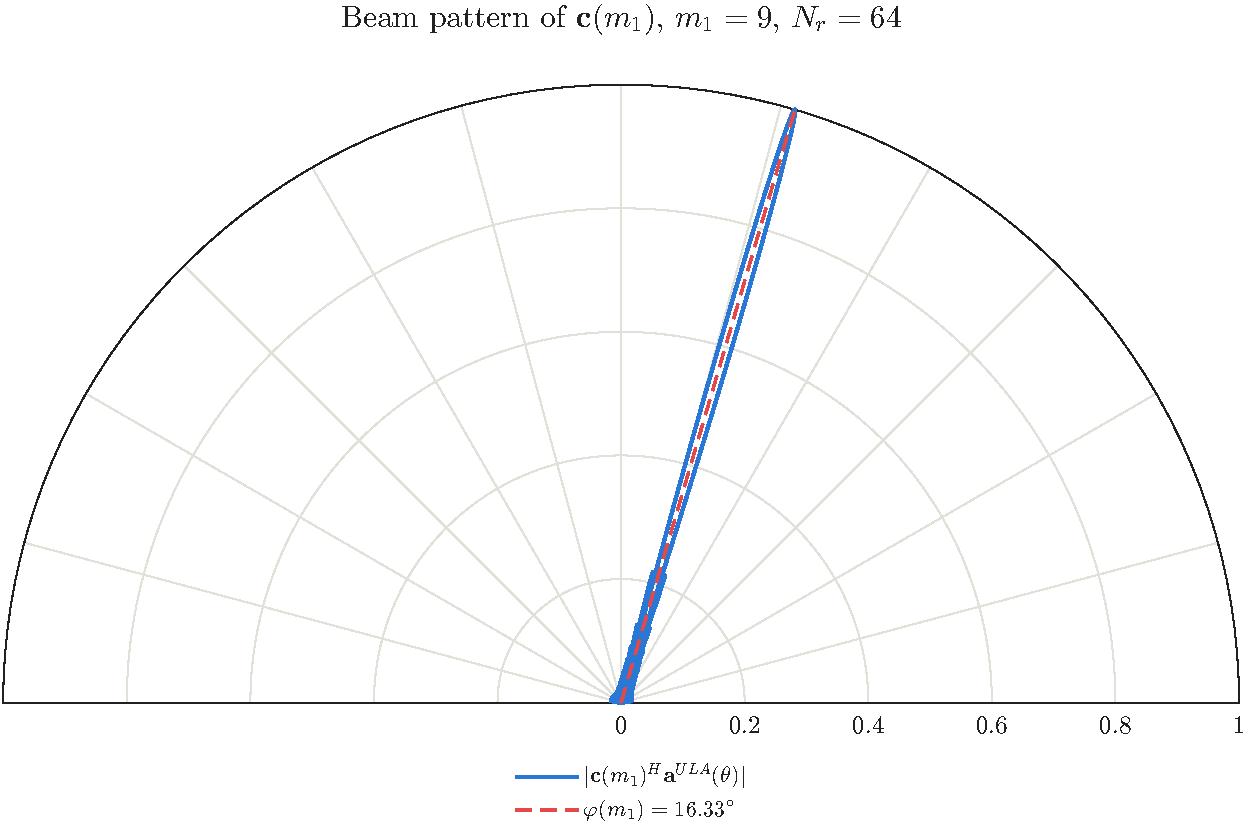
\includegraphics[width=0.78\linewidth]{q1b.pdf}
    \caption{Beam Pattern $|\mathbf{c}(m_1)^H\mathbf{a}^{ULA}(\theta)|$ for $m_1 = 9$ in Polar Coordinates}
\end{figure}

\newpage

\section{(c) Combiner Output versus $m$}

\question{Please check the magnitude of the combination result, $|\mathbf{c}(m)^H\mathbf{h}|$ versus $m$. Draw the figure
with x-axis indicating the value of $m$ and y-axis is the magnitude of $|\mathbf{c}(m)^H\mathbf{h}|$ for
$m = -32, -31, \ldots, 31$. (10\%)}

\begin{figure}[H]
    \centering
    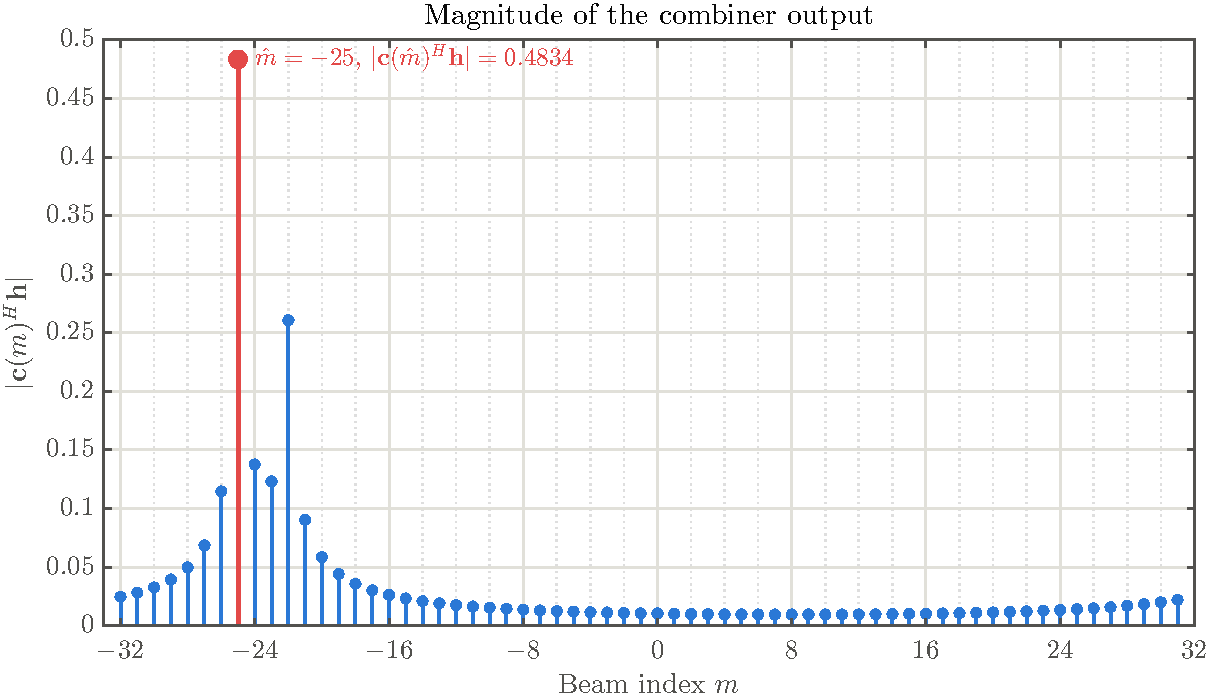
\includegraphics[width=0.9\linewidth]{q1c.pdf}
    \caption{Magnitude of the Combiner Output $|\mathbf{c}(m)^H\mathbf{h}|$ for $m = -32 \sim 31$}
\end{figure}

The output is large only for $m = -25 \sim -21$, where the two paths arrive: 0.4834 at $m = -25$ and a second peak of
0.2608 at $m = -22$. On the beam-index axis, path 1 lies at $N\sin\theta_{r,1}/2 = -24.73$ and path 2 at $-22.40$.
Neither is an integer, so some power leaks into the neighboring beams.

\section{(d) Nominal Pointing Angle of the Selected Beam}

\question{If $\hat m = \arg\max_m |\mathbf{c}(m)^H\mathbf{H}_1|$, then calculate the nominal pointing angle
$\varphi(\hat m)$ associated with the beamforming vector $\mathbf{c}(\hat m)$ (5\%). Please check the differences of
$|\varphi(\hat m) - \theta_{r,1}|$ and $|\varphi(\hat m) - \theta_{r,2}|$. (5\%)}

Here $\mathbf{H}_1$ is the vector $\mathbf{h}$ from (a). From (c), $\hat m = -25$ and
\begin{align}
    \varphi(\hat m) &= \sin^{-1}\!\Big(\frac{2 \times (-25)}{64}\Big) = -0.896666\ \text{rad} = -51.3752^\circ, \\
    |\varphi(\hat m) - \theta_{r,1}| &= 0.013191\ \text{rad} = 0.7558^\circ, \\
    |\varphi(\hat m) - \theta_{r,2}| &= 0.121197\ \text{rad} = 6.9441^\circ .
\end{align}

\section{(e) Which Path Does the Selected Beam Follow?}

\question{Explain whether the selected beam is closer to the stronger path, the weaker path, or neither. Support the
explanation using the path magnitudes, path phases, angular separation, and the values. (5\%)}

The selected beam is closer to the stronger path, path 1. Table~\ref{tab:q1e} splits
$\mathbf{c}(\hat m)^H\mathbf{h}$ into the contribution of each path,
$\frac{\alpha_l}{\sqrt 2}\,\mathbf{c}(\hat m)^H\mathbf{a}^{ULA}(\theta_{r,l})$.

\begin{table}[H]
\centering
\caption{Contribution of Each Path to the Selected Beam $\hat m = -25$}
\label{tab:q1e}
\setlength{\tabcolsep}{7pt}
\renewcommand{\arraystretch}{1.2}
\begin{tabular}{ccccccc}
\toprule
Path & $|\alpha_l|$ & $\angle\alpha_l$ & $N\sin\theta_{r,l}/2$ & $|\mathbf{c}(\hat m)^H\mathbf{a}(\theta_{r,l})|$ &
$|\text{contribution}|$ & $\angle\text{contribution}$ \\
\midrule
1 & 0.7329 & $+21.33^\circ$ & $-24.73$ & 0.8879 & 0.4601 & $-25.74^\circ$ \\
2 & 0.4313 & $+125.71^\circ$ & $-22.40$ & 0.1170 & 0.0357 & $+25.31^\circ$ \\
\bottomrule
\end{tabular}
\end{table}

Path 1 is the stronger one ($|\alpha_1| = 0.733$ vs.\ $|\alpha_2| = 0.431$). The two paths are $6.19^\circ$ apart, which
is 2.33 beam spacings and wider than the $5.75^\circ$ null-to-null width of beam $-25$, so each path has its own best
beam: path 1 is 0.27 beam
from $m = -25$ and path 2 is 0.40 beam from $m = -22$. In beam $-25$, path 1 keeps a gain of 0.888, while path 2 only
leaks in through a sidelobe (0.117), so its contribution is 0.0357 against 0.4601. The two contributions are
$51^\circ$ apart in phase, so their sum, 0.4834, exceeds 0.4601 by 0.0233. A term of 0.036
cannot move the maximum, whatever its phase. The best beam for path 2, $m = -22$, reaches 0.2608.

\newpage

% ─────────────────────────────────────────────
\chapter{Q2 — Symbol Timing by Delay-and-Correlate}
% ─────────────────────────────────────────────
\question{Please download ``hw4.mat'' from the NTUCool. Use ``load hw4.mat'' to retrieve the original data. It contains
one variable ``OFDMTx'', which are the complex time-domain discrete signals generated by OFDM baseband transmitter.
There are 32 samples in cyclic prefix ($N_g = 32$) and the FFT size is 128 ($N = 128$). The first OFDM symbol is a
preamble which has identical two repetitions as below, and then three normal OFDM symbols follows the preamble. Assume
the received signal $z_m$ equal to the transmitted signal. If $m \le 0$, $z_m = 0$.}

\texttt{OFDMTx} has 640 samples, four symbols of $N_g + N = 160$ samples. The preamble, CP included, is periodic with
period $N/4 = 32$: the script finds samples 33--64, 65--96, 97--128 and 129--160 identical, and the CP equals 129--160.
Indices start from 1, so symbol $s$ ends at sample $160s$.

\section{(a) $\Phi_{DC}(m)$ with $R = 64$, $L = 64$}

\question{Please draw magnitude of the delay and correlate result $\Phi_{DC}(m)$ by setting $R = 64$ and $L = 64$, for
$m = 1, \ldots, 640$ where
\[ \Phi_{DC}(m) = \Big|\sum_{r=0}^{R-1} z_{m-r}\,z^*_{m-r-L}\Big| . \quad (10\%) \]
(Mark the X and Y value of the peak in the figure. The first index in the figure is 1.)}

\begin{figure}[H]
    \centering
    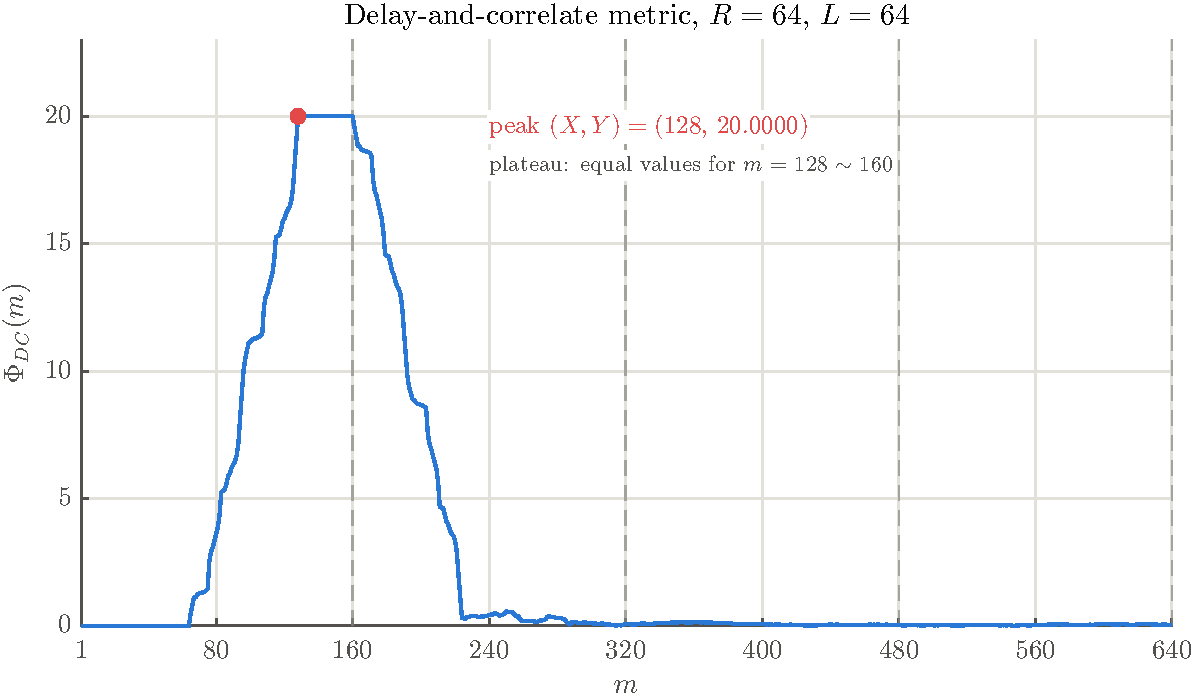
\includegraphics[width=0.9\linewidth]{q2a.pdf}
    \caption{$\Phi_{DC}(m)$ for $R = L = 64$, $m = 1 \sim 640$ (dashed lines: symbol boundaries)}
\end{figure}

The peak is at $(X, Y) = (128,\ 20.0000)$. $\Phi_{DC}$ is 0 for $m \le 64$ because $z_{m-r-64} = 0$ there, rises while
the delayed window moves into the preamble, stays at 20 for $m = 128 \sim 160$, and drops once the window reaches the
data symbols.

\section{(b) Detected Timing and Plateau in the First Symbol}

\question{Consider only the first symbol for $1 \le m \le 160$. If a decision is made according to $\hat m_{DC} =
\arg\max \Phi_{DC}(m)$, what's the detected timing in the first symbol? (5\%) Whether a plateau will be seen or not in
the waveform of $\Phi_{DC}(m)$ using the setting in Q2(a)? Why? (5\%)}

The detected timing is $\hat m_{DC} = 128$ with $\Phi_{DC} = 20$, the first sample of the maximum: all 33 samples
from 128 to 160 have the same value, and \texttt{max} returns the first of them. The preamble ends at 160.

$\Phi_{DC}$ shows a plateau. $\Phi_{DC}(m)$ uses the 128 samples $z_{m-127}, \ldots, z_m$. If all of them lie inside the
periodic preamble ($m - 127 \ge 1$ and $m \le 160$), every product is $z_{m-r}z^*_{m-r-64} = |z_{m-r}|^2$, because the
lag 64 is a multiple of the period 32. Then
\begin{equation}
    \Phi_{DC}(m) = \sum_{r=0}^{63} |z_{m-r}|^2 = 20, \qquad 128 \le m \le 160,
\end{equation}
and the value stays constant because a 64-sample window covers two full periods. The plateau is
$160 - (R + L) + 1 = 33$ samples long, which is positive because the repeated part (160 samples, CP included) is longer
than $R + L = 128$. At $m = 161$ the first data sample enters and the value drops to 19.56.

\newpage

\section{(c) $\Phi_{DC}(m)$ and $\Phi_{NM}(m)$ with $R = 32$, $L = 128$}

\question{Discard the first symbol. Now, the signal length is 480 sample. Please draw the result $\Phi_{NM}(m)$ and
$\Phi_{DC}(m)$ by setting $R = 32$ and $L = 128$ for $m = 1, \ldots, 480$. If a decision is made according to
$\hat m_{DC} = \arg\max \Phi_{DC}(m)$ and $\hat m_{NM} = \arg\max \Phi_{NM}(m)$ every symbol, what are the results?
Please explain the decision difference between $\Phi_{NM}(m)$ and $\Phi_{DC}(m)$. (15\%)
\[ \Phi_{NM}(m) = \frac{\big|\sum_{r=0}^{R-1} z_{m-r}\,z^*_{m-r-L}\big|^2}{\big(\sum_{r=0}^{R-1} |z_{m-r}|^2\big)^2} \]}

With $R = N_g$ and $L = N$, the window compares the last 32 samples of a symbol with its CP, so the exact match is at
$m = 160, 320, 480$. I take ``every symbol'' as the blocks $m = 1 \sim 160$, $161 \sim 320$ and $321 \sim 480$.

\begin{figure}[H]
    \centering
    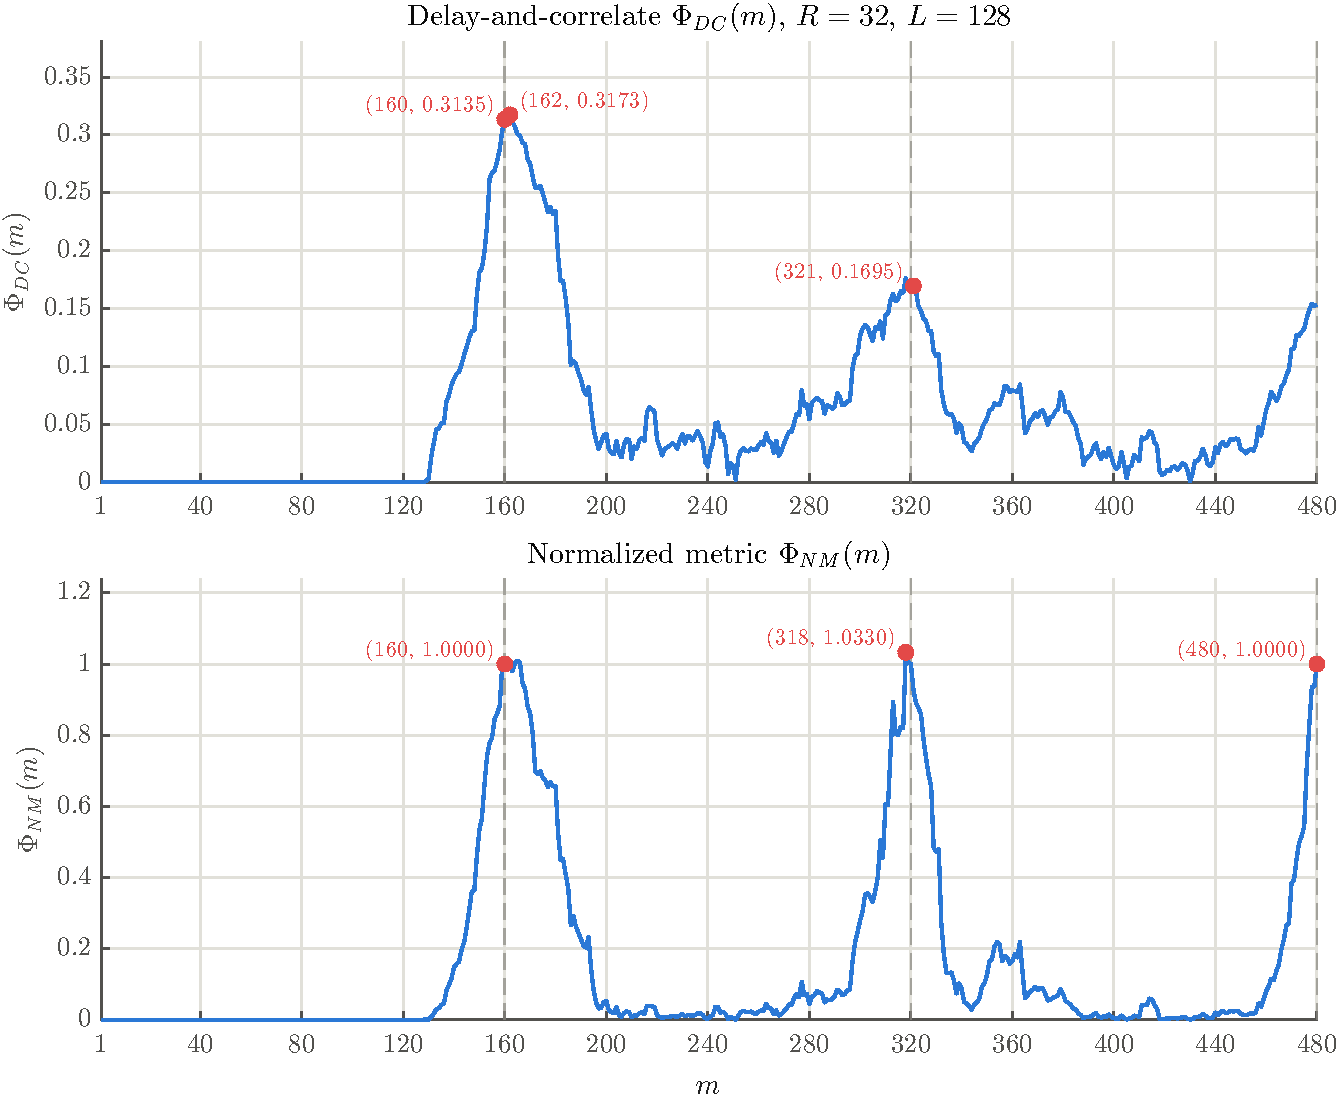
\includegraphics[width=0.9\linewidth]{q2c.pdf}
    \caption{$\Phi_{DC}(m)$ (top) and $\Phi_{NM}(m)$ (bottom) for $R = 32$, $L = 128$, with the Maximum of Every Symbol}
\end{figure}

\begin{table}[H]
\centering
\caption{Decision in Every Symbol (Noiseless)}
\setlength{\tabcolsep}{9pt}
\renewcommand{\arraystretch}{1.2}
\begin{tabular}{cccccc}
\toprule
Symbol & Block & Symbol end & $\hat m_{DC}$ ($\Phi_{DC}$) & $\hat m_{NM}$ ($\Phi_{NM}$) & $\sum_r|z_{m-r}|^2$ at symbol end \\
\midrule
1 & $1 \sim 160$   & 160 & 160 (0.3135) & 160 (1.0000) & 0.3135 \\
2 & $161 \sim 320$ & 320 & 162 (0.3173) & 318 (1.0330) & 0.1680 \\
3 & $321 \sim 480$ & 480 & 321 (0.1695) & 480 (1.0000) & 0.1532 \\
\bottomrule
\end{tabular}
\end{table}

At the symbol end every product is $|z|^2$, so $\Phi_{DC}$ there equals the energy of the window, and that energy differs
between symbols (0.3135, 0.1680, 0.1532). Symbol 1 is the strongest. The falling edge of its lobe is still 0.3173 at
$m = 162$, above the true peak of symbol 2 (0.1680), so block 2 picks 162, which belongs to the previous boundary.
Block 3 fails the same way: 321 is the tail of the symbol-2 lobe (0.1695) and beats the symbol-3 peak (0.1532), so
$\Phi_{DC}$ finds symbol 1 alone.

$\Phi_{NM}$ divides by the squared window energy, so an exact CP match gives 1 for every symbol, whatever its power.
It finds 160 and 480. In block 2 it picks 318 with $\Phi_{NM} = 1.033$, two samples early. $\Phi_{NM}$ can exceed
1 because the denominator only uses the current window: by Cauchy--Schwarz,
$\Phi_{NM}(m) \le \sum_r |z_{m-r-L}|^2 / \sum_r |z_{m-r}|^2$, and this ratio is above 1 whenever the delayed window
carries more energy. The decisions therefore differ because $\Phi_{DC}$ depends on the symbol power and
$\Phi_{NM}$ does not.

\newpage

\section{(d) $\Phi_{NM}(m)$ at SNR = 12 dB}

\question{Now, add noise by yourself. The SNR is 12dB. Please use normalized metric $\Phi_{NM}(m)$ to perform symbol
timing detection again. Report the detected result $\hat m_{NM} = \arg\max \Phi_{NM}(m)$ every symbol and compare the
results to the answer in Q2(c). Please explain the difference if any. (10\%)}

I add circular complex Gaussian noise to the 480-sample record with $\sigma^2 = P_s/10^{1.2}$, where
$P_s = \overline{|z_m|^2} = 0.007585$ is the record power, so $\sigma^2 = 4.79 \times 10^{-4}$ (seed 11407439). The SNR
measured on this realization is 12.07\,dB.

\begin{figure}[H]
    \centering
    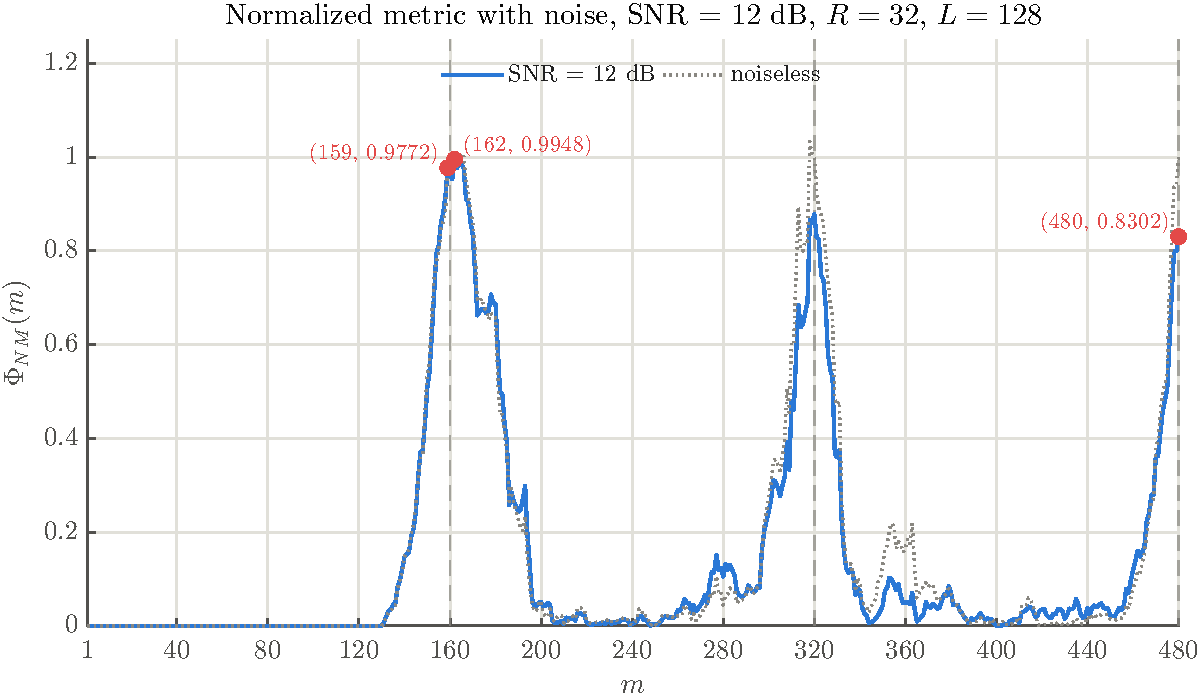
\includegraphics[width=0.9\linewidth]{q2d.pdf}
    \caption{$\Phi_{NM}(m)$ at SNR = 12 dB (blue) and Noiseless (dotted), with the Maximum of Every Symbol}
\end{figure}

\begin{table}[H]
\centering
\caption{Decision of $\Phi_{NM}$ in Every Symbol, SNR = 12 dB versus Noiseless}
\setlength{\tabcolsep}{12pt}
\renewcommand{\arraystretch}{1.2}
\begin{tabular}{ccccc}
\toprule
Symbol & $\hat m_{NM}$ at 12 dB ($\Phi_{NM}$) & $\hat m_{NM}$ in Q2(c) & $\Phi_{NM}$ at symbol end, 12 dB & Local SNR \\
\midrule
1 & 159 (0.9772) & 160 & 0.9643 & 13.1 dB \\
2 & 162 (0.9948) & 318 & 0.8784 & 10.4 dB \\
3 & 480 (0.8302) & 480 & 0.8302 & 10.0 dB \\
\bottomrule
\end{tabular}
\end{table}

Symbol 3 is unchanged, symbol 1 moves one sample earlier, and symbol 2 is now wrong. With noise the CP and its copy no
longer match, and the peak drops to about $\big(S/(S + \sigma^2)\big)^2$, where $S$ is the signal power in the
window. The noise power is the same everywhere, but the CP windows carry different power, so the local SNR is 13.1, 10.4
and 10.0\,dB and the expected peaks are about 0.91, 0.84 and 0.83. The measured values at the symbol ends (0.964, 0.878,
0.830) follow the same order.

The lower peak breaks symbol 2. Its value drops to 0.878, while the falling edge of the symbol-1 lobe at $m = 162$, which
has the highest local SNR, stays at 0.995. Both lie in block 2, so the argmax returns 162, the same mistake $\Phi_{DC}$
made in Q2(c). Each lobe is $2R$ wide and centered on a block edge, so half of each lobe falls into the next block.
Symbol 1 moves to 159 because the top of its lobe is almost flat (0.977 vs.\ 0.964) and the noise picks the winner.

\newpage

% ─────────────────────────────────────────────
\chapter{Q3 — Hardware Symbol Boundary Detector}
% ─────────────────────────────────────────────
\question{Now, we aim to implement $\Phi_{NM}(m)$. A constant threshold $\eta$ is set to activate the peak searcher. It
means the local maximum will be searched only when the correlation output is larger than $\eta$, namely
\[ \Phi_{NM}(m) = \frac{\big|\sum_{r=0}^{R-1} z_{m-r}\,z^*_{m-r-L}\big|^2}{\big(\sum_{r=0}^{R-1} |z_{m-r}|^2\big)^2} > \eta . \]
The delay correlation is implemented for the numerator as in the following.
\begin{center}
    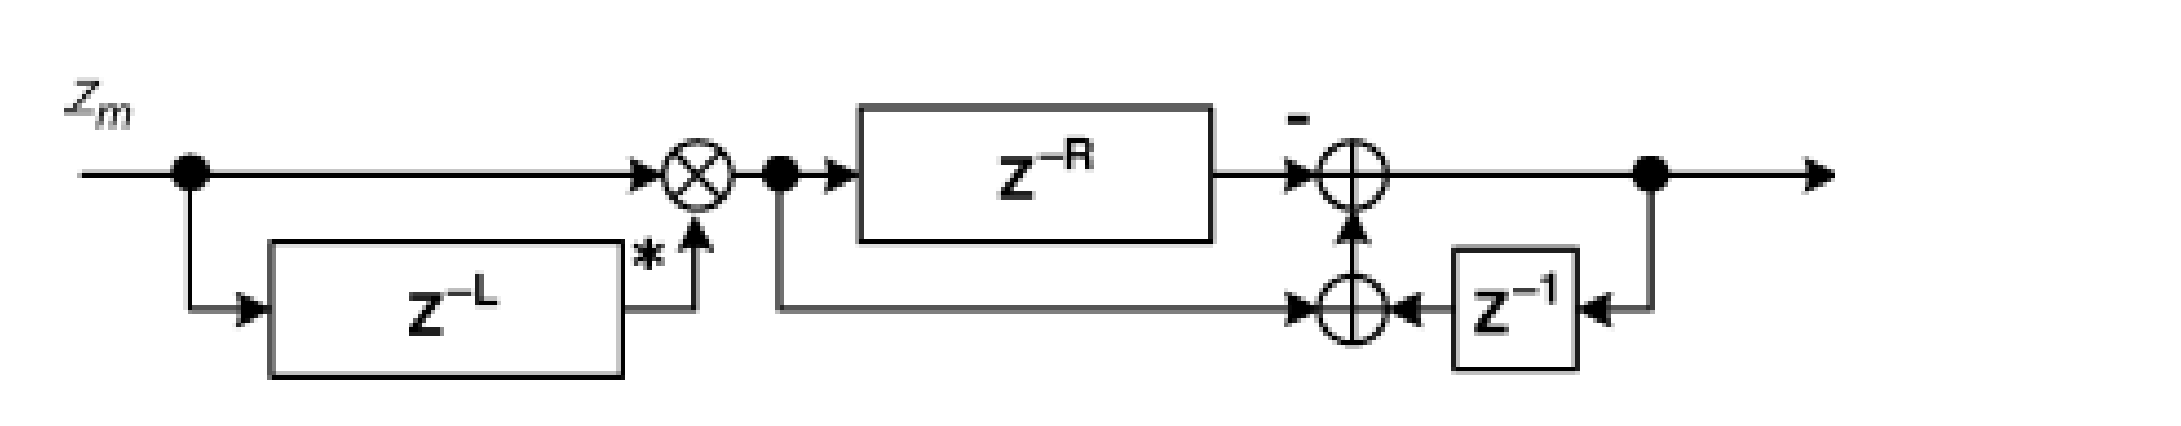
\includegraphics[width=0.62\linewidth]{q3_dc.png}
\end{center}}

The metric above follows the TA's correction, which replaced the original
$\Phi_{NM}(m) = \big|\sum_{r=0}^{R-1} z_{m-r}z^*_{m-r-L}\big|$ with the normalized metric of Q2(c). The hardware uses the
setting of Q2(c), $R = 32$ and $L = 128$, on the 480-sample record, with one input sample per clock cycle.

\section{(a) Threshold $\eta$}

\question{Decide your own setting of $\eta$ from the given signals and the signals with SNR equal to 12dB. Please report
the setting and explain the reason. (5\%)}

I set $\eta = 0.52$, stored as the U2.14 code 8520 (\texttt{0x2148}).

Around each boundary $\Phi_{NM}$ forms a lobe $2R$ samples wide ($|m - 160k| < R$, shaded in the figure below). The top
of each lobe must pass $\eta$, and the values outside the lobes must stay below it, otherwise the peak searcher starts
on data samples.

\begin{table}[H]
\centering
\caption{$\Phi_{NM}$ inside and outside the Lobes}
\setlength{\tabcolsep}{10pt}
\renewcommand{\arraystretch}{1.2}
\begin{tabular}{lcc}
\toprule
Signal & Lobe peaks (symbol 1, 2, 3) & Max.\ outside the lobes \\
\midrule
Given signal (noiseless) & 1.0092, 1.0330, 1.0000 & 0.2328 \\
12 dB, record of Q2(d) & 0.9948, 0.8784, 0.8302 & 0.2987 \\
12 dB, 2000 runs: min.\ peak / max.\ outside & 0.6913, 0.6220, 0.5669 & 0.4831 \\
12 dB, 2000 runs: 0.1\% / 99.9\% quantile & 0.7141, 0.6301, 0.5796 & 0.4614 \\
\bottomrule
\end{tabular}
\end{table}

For the given signal any $\eta$ between 0.24 and 1.0 works, and the noisy record of Q2(d) still leaves a gap from 0.30
to 0.83. One noisy record says little about other noise realizations, so I also ran 2000 of them at 12\,dB. The lobe
peaks then fall to 0.567 and the largest value outside the lobes rises to 0.483. I place $\eta$ halfway between the
99.9\% quantile outside the lobes and the 0.1\% quantile of the peaks:
\begin{equation}
    \eta = \frac{0.461 + 0.580}{2} \approx 0.52 .
\end{equation}
Over the 2000 runs this leaves margins of 0.047 below the lowest peak and 0.037 above the highest outside value, and
each run gives three detections with the peak searcher of (d).

\begin{figure}[H]
    \centering
    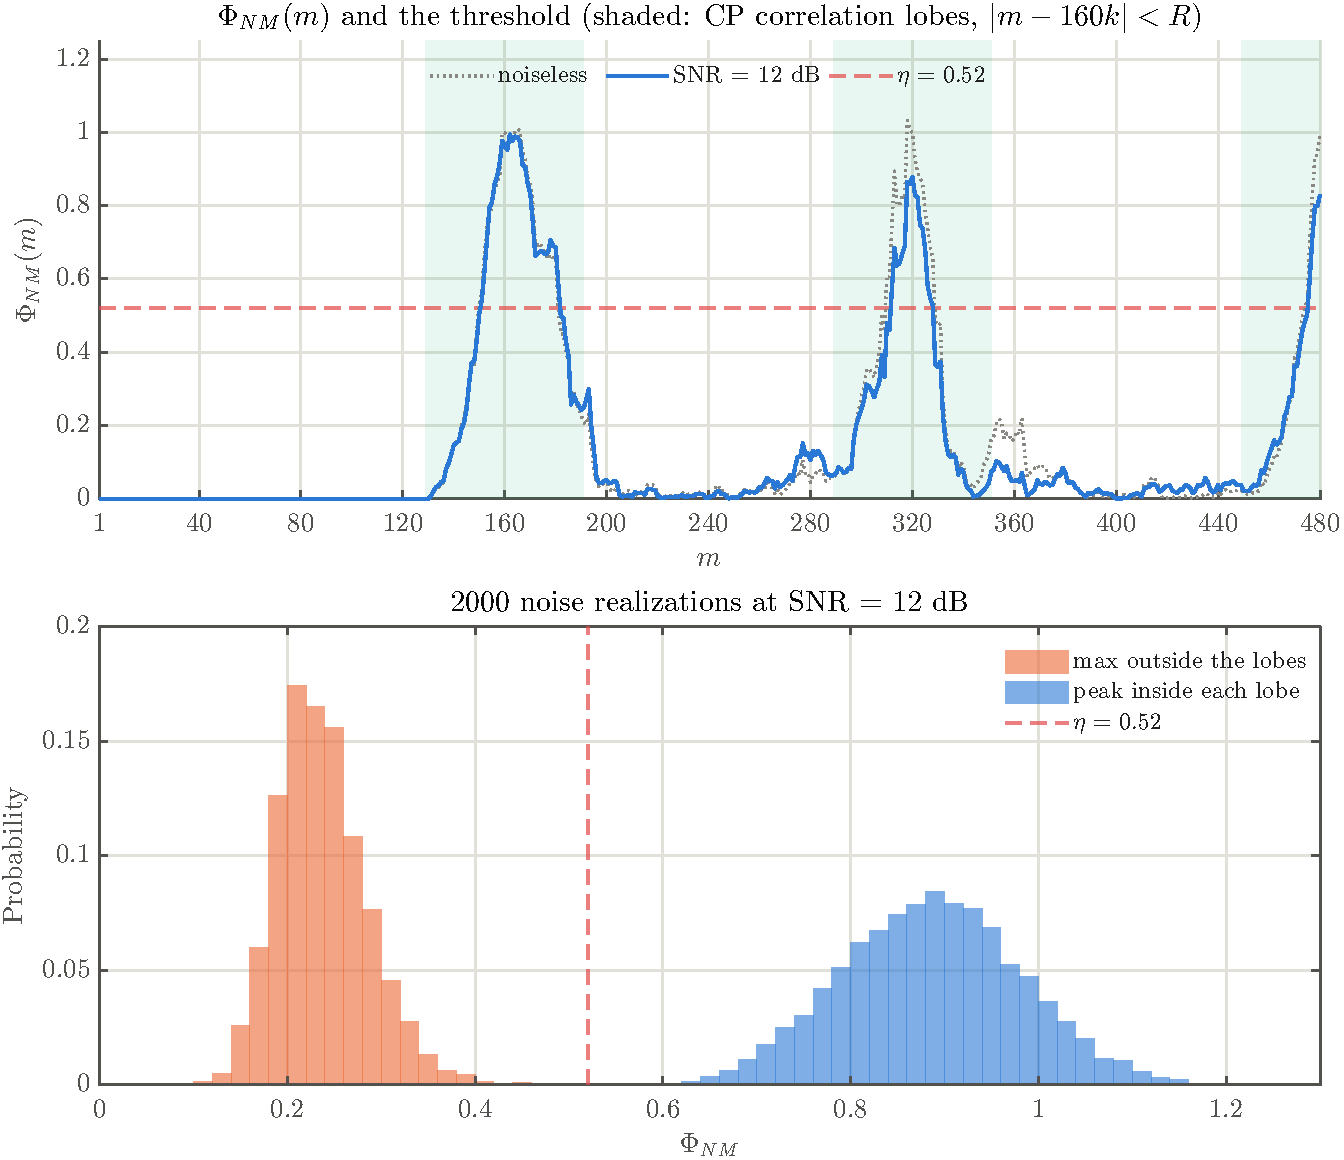
\includegraphics[width=0.86\linewidth]{q3a.pdf}
    \caption{$\Phi_{NM}(m)$ with $\eta = 0.52$ (top) and the Distribution of the Lobe Peaks and of the Largest Value outside the Lobes over 2000 Noise Realizations (bottom)}
\end{figure}

\newpage

\section{(b) Block Diagram}

\question{Assume that the complex input signal enters one by one sequentially. Draw the block diagram of your design for
the threshold-judgement module, divider, and the peak searcher together with the delay correlator. Connect all these
modules together in one figure. (10\%)}

\begin{figure}[H]
    \centering
    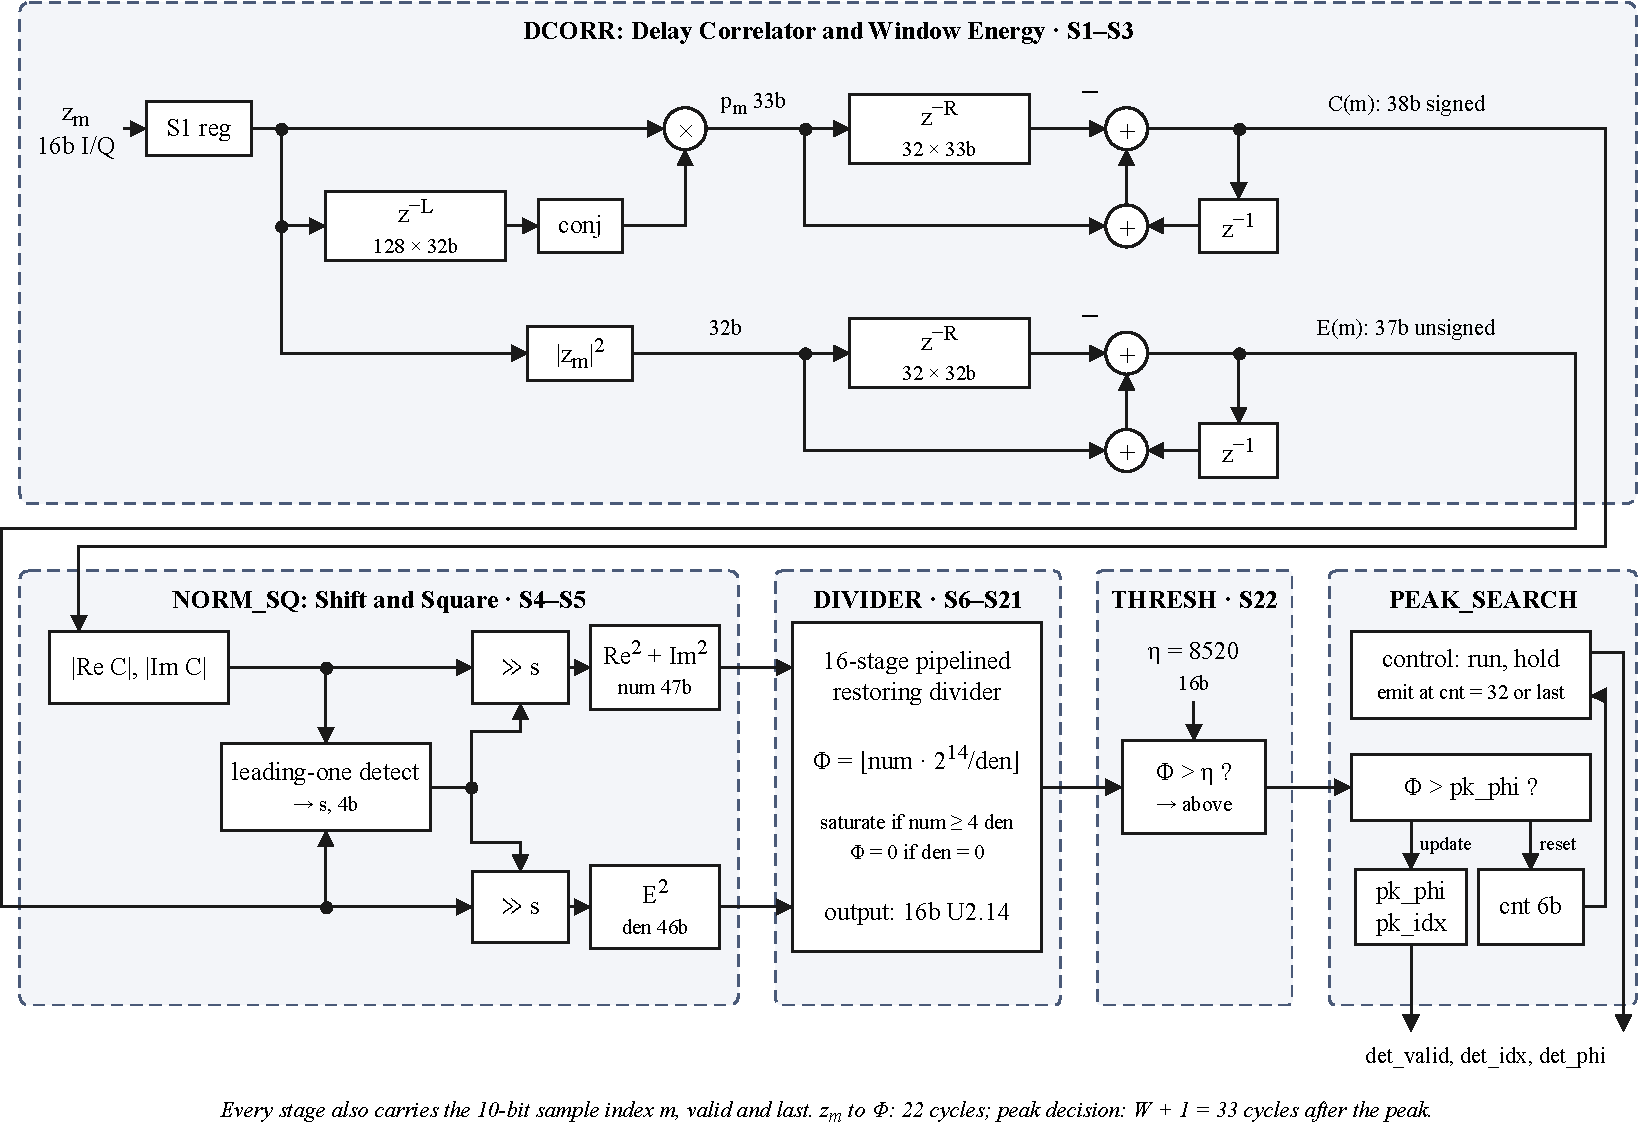
\includegraphics[width=\linewidth]{q3b.pdf}
    \caption{Block Diagram of the Symbol Boundary Detector}
    \label{fig:q3b}
\end{figure}

One sample $z_m$ (16-bit I and Q) enters per clock cycle. \texttt{DCORR} follows the recursive structure of the
question, $C(m) = C(m-1) + p_m - p_{m-R}$ with $p_m = z_m z^*_{m-L}$, and a second accumulator of the same form builds
the energy $E(m)$. The sample index $m$ travels down the pipeline with the data, so each output carries the index of its
own sample.

\newpage

\section{(c) Word Lengths}

\question{Please quantize your input signal $z_m$ by 16 bits. To avoid overflow, please explain the wordlength setting
of your accumulator and your divider. (5\%)}

After the preamble, the largest $|\mathrm{Re}\,z_m|$ or $|\mathrm{Im}\,z_m|$ is 0.223, noise included. I quantize I and
Q to 16-bit two's complement with 16 fraction bits, $z_q = \mathrm{round}(z \cdot 2^{16})$, which covers $[-0.5, 0.5)$
with an LSB of $2^{-16}$. The scale factor cancels in the ratio $\Phi_{NM}$, so it sets the resolution of the metric.

The word lengths below follow from the worst-case input $|\mathrm{Re}\,z|, |\mathrm{Im}\,z| \le 2^{15}$ (LSB units).

\begin{table}[H]
\centering
\caption{Word Lengths}
\setlength{\tabcolsep}{8pt}
\renewcommand{\arraystretch}{1.25}
\begin{tabular}{l c >{\raggedright\arraybackslash}p{0.5\linewidth}}
\toprule
Signal & Bits & Reason \\
\midrule
$z_m$ (I, Q) & 16 signed & given \\
$\mathrm{Re}/\mathrm{Im}\{z_m z^*_{m-L}\}$ & 33 signed & sum of two $16 \times 16$ products, $|ac + bd| \le 2^{31}$ \\
$|z_m|^2$ & 32 unsigned & $a^2 + b^2 \le 2^{31}$ \\
Accumulator $C(m)$ & 38 signed & $R = 32$ terms add $\log_2 R = 5$ bits \\
Accumulator $E(m)$ & 37 unsigned & same, from 32 bits \\
After the common shift & 23 & top 23 bits of the largest of $|\mathrm{Re}\,C|$, $|\mathrm{Im}\,C|$, $E$ \\
Numerator $|C|^2$ & 47 unsigned & $2 \times 23 + 1$ \\
Denominator $E^2$ & 46 unsigned & $2 \times 23$ \\
Dividend $\mathrm{num} \cdot 2^{14}$ & 61 & also the partial remainder of each divider stage \\
Quotient $\Phi$ & 16 unsigned & U2.14, range $[0, 4)$, LSB $2^{-14}$ \\
\bottomrule
\end{tabular}
\end{table}

\textbf{Accumulator.} With 38 and 37 bits the accumulators hold the full sum of 32 worst-case terms, so they cannot
overflow. In the recursive form $C(m) = C(m-1) + p_m - p_{m-R}$ the register equals the true window sum after each
update.

\textbf{Divider.} Squaring the full sums would need 73-bit operands. Scaling $C$ and $E$ by the same factor leaves
$\Phi_{NM}$ unchanged, so \texttt{NORM\_SQ} shifts all three values right by $s = \max(0, \text{msb} - 22)$, where
msb is the leading-one position of the largest one. The divider then works on 47/46-bit operands. The quotient needs
two integer bits because $\Phi_{NM}$ can exceed 1 (1.033 in Q2(c)). It saturates to $4 - 2^{-14}$ if
$\mathrm{num} \ge 4\,\mathrm{den}$ and outputs 0 if $\mathrm{den} = 0$, so it cannot overflow either. On the given data
the largest shift is 8, and the hardware metric differs from the floating-point $\Phi_{NM}$ by at most
$7.2 \times 10^{-5}$ (noiseless) and $9.3 \times 10^{-5}$ (12\,dB), i.e.\ at most 1.5 LSB.

\newpage

\section{(d) HDL Implementation and Simulation}

\question{Implement your design by hardware description language (HDL) (20\%). Explain the latency of your local peak
searcher (5\%). Show the behavior simulation results (timing diagram) of your symbol boundary detector (10\%). Please
compare your implementation results with your simulation result in Q3(c) and provide your comment. (5\%)}

\subsection{Implementation}

I wrote the design in SystemVerilog (\texttt{01\_src/02\_RTL}) with the modules of Figure~\ref{fig:q3b}. The
pipeline from input to metric is:
\begin{center}
\setlength{\tabcolsep}{8pt}
\renewcommand{\arraystretch}{1.2}
\begin{tabular}{lll}
\toprule
Stage & Module & Operation \\
\midrule
S1 & \texttt{DCORR} & input register, sample index counter \\
S2 & \texttt{DCORR} & $z^{-L}$ delay line, $z_m z^*_{m-L}$ and $|z_m|^2$ \\
S3 & \texttt{DCORR} & $z^{-R}$ delay line, recursive sums $C(m)$, $E(m)$ \\
S4 & \texttt{NORM\_SQ} & leading-one detection and common shift \\
S5 & \texttt{NORM\_SQ} & squares $|C|^2$, $E^2$ \\
S6 -- S21 & \texttt{DIVIDER} & 16 restoring stages, one quotient bit each \\
S22 & \texttt{THRESH} & $\Phi > \eta$ \\
\bottomrule
\end{tabular}
\end{center}
$\Phi(m)$ leaves \texttt{THRESH} 22 cycles after $z_m$ enters, and one new value comes out every cycle.

The peak searcher processes one metric sample per cycle:
\begin{enumerate}[label=(\arabic*), leftmargin=1.6em]
    \item When idle and $\Phi(m) > \eta$, it starts a search with candidate $(m, \Phi(m))$ and counter 0.
    \item While searching, a value above $\eta$ that is larger than the candidate replaces it and resets the counter.
    Any other sample increases the counter.
    \item When the counter reaches $W = 32$, it outputs the candidate (\texttt{det\_valid}, \texttt{det\_idx}) and
    becomes idle. A new search needs $\Phi \le \eta$ first, so each lobe gives one detection.
    \item At the last sample of the record (\texttt{in\_last}), a running search is output at once.
\end{enumerate}
I use $W = R = 32$ because a lobe extends $R$ samples on each side of its peak; after 32 samples without a larger value
the search has left the lobe.

\subsection{Latency of the Local Peak Searcher}

The searcher can call a value the local maximum only after it sees the following samples. The searcher waits
$W = 32$ metric samples and then registers the result, so \texttt{det\_valid} rises
\begin{equation}
    \underbrace{W}_{32\ \text{samples}} + \underbrace{1}_{\text{output register}} = 33\ \text{cycles}
\end{equation}
after $\Phi(\hat m)$ reaches the searcher, or $22 + 33 = 55$ cycles after $z_{\hat m}$ enters the design. The
simulation measures 55 cycles for the boundaries 165 and 318 of the noiseless case and 162 and 320 of the 12\,dB case.
For the last boundary, $m = 480$, the flush rule outputs the candidate one cycle after the last sample. The waveforms in
the next subsection show these cases for the noiseless record.

\subsection{Behavioral Simulation}

\texttt{q3.m} writes the quantized inputs, $\eta$ and the bit-true golden data into \texttt{01\_TESTBED/src}.
\texttt{PATTERN.sv} feeds the 480 samples of each case, one per cycle, and compares every metric sample and every
detection with the golden data. In Synopsys VCS S-2021.09, both the noiseless and the 12\,dB case match the bit-true
model for all 480 metric samples and all 3 detections.

The waveforms below are the noiseless case in Verdi, with a 10\,ns clock. \texttt{cnt} is the counter inside
\texttt{PEAK\_SEARCH}. It is a register, so it shows the update one cycle after the metric sample that caused it. After a detection it
stays at 32 until the next search starts.

\begin{figure}[H]
    \centering
    \begin{subfigure}{\linewidth}
        \centering
        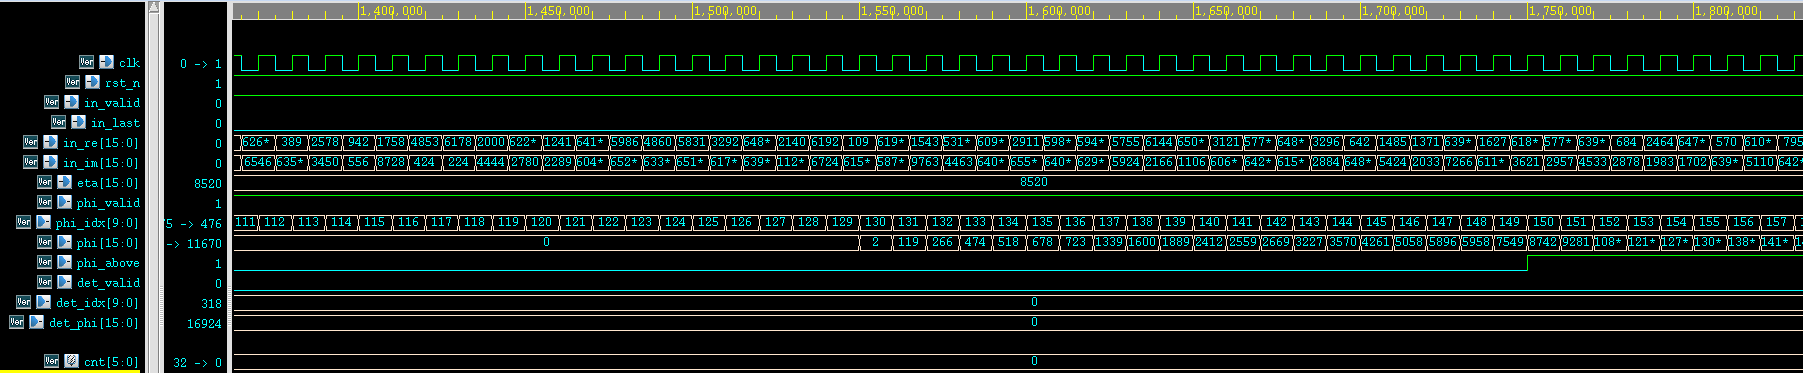
\includegraphics[width=\linewidth]{q3d_wave2.png}
        \caption{\texttt{phi\_above} rises at $m = 150$, where $\Phi = 8742 > \eta$.}
    \end{subfigure}
    \par\medskip
    \begin{subfigure}{\linewidth}
        \centering
        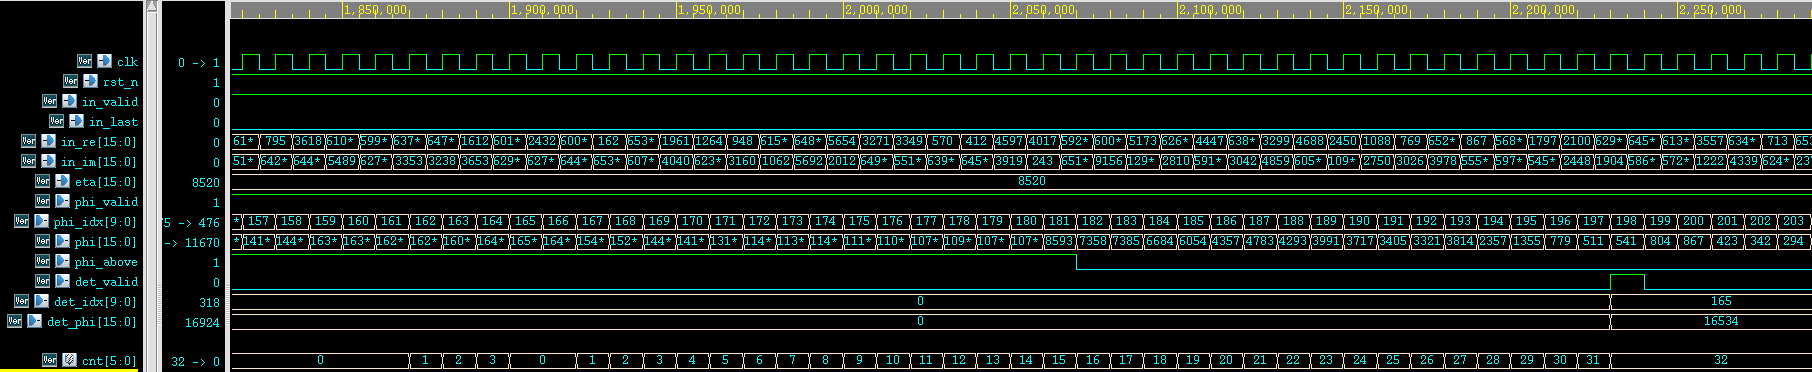
\includegraphics[width=\linewidth]{q3d_wave3.png}
        \caption{\texttt{cnt} counts from 0 to 32 after the candidate $m = 165$; \texttt{det\_valid} rises at
        \texttt{phi\_idx} = 198.}
    \end{subfigure}
    \caption{Behavioral Simulation: First Boundary, $\hat m = 165$}
    \label{fig:q3d_b1}
\end{figure}

In Figure~\ref{fig:q3d_b1}, $\Phi$ crosses $\eta$ at $m = 150$ and the search starts. Every larger value replaces the
candidate and resets \texttt{cnt}; the last replacement is $m = 165$ with $\Phi = 16534$ (1.0092). From there
\texttt{cnt} runs from 0 to 32 without another reset, \texttt{phi\_above} falls at $m = 182$ ($\Phi = 7358$), and
\texttt{det\_valid} rises with \texttt{det\_idx} = 165 and \texttt{det\_phi} = 16534 while \texttt{phi\_idx} is 198,
i.e.\ $198 - 165 = 33$ cycles after the candidate.

\begin{figure}[H]
    \centering
    \begin{subfigure}{\linewidth}
        \centering
        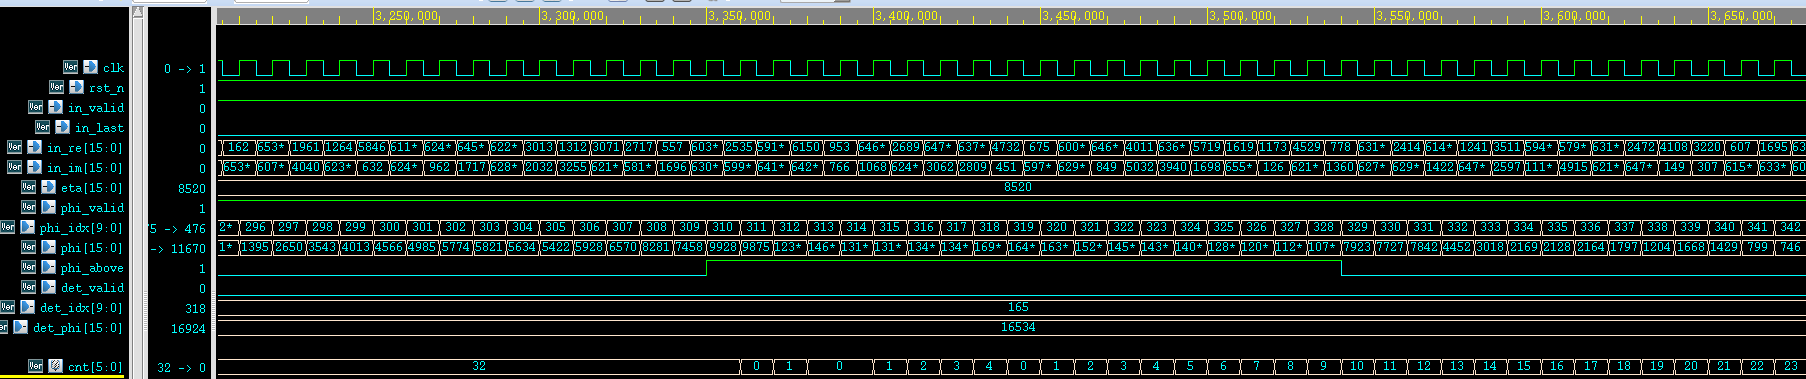
\includegraphics[width=\linewidth]{q3d_wave4.png}
        \caption{\texttt{phi\_above} rises at $m = 310$; the candidate is replaced several times, last at $m = 318$.}
    \end{subfigure}
    \par\medskip
    \begin{subfigure}{\linewidth}
        \centering
        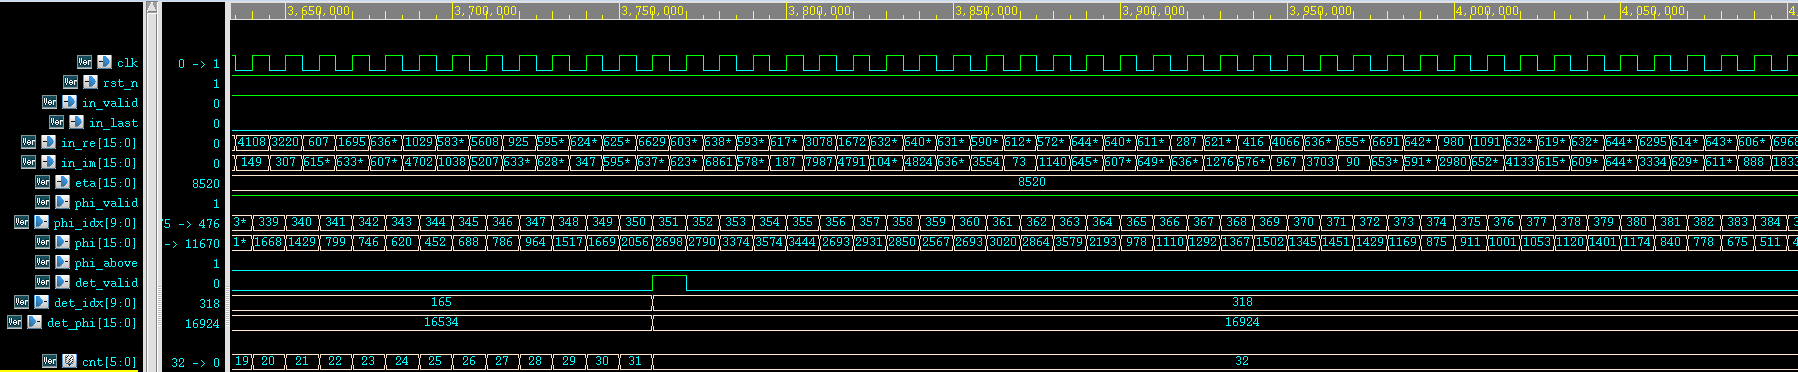
\includegraphics[width=\linewidth]{q3d_wave5.png}
        \caption{\texttt{cnt} reaches 32 and \texttt{det\_valid} rises at \texttt{phi\_idx} = 351.}
    \end{subfigure}
    \caption{Behavioral Simulation: Second Boundary, $\hat m = 318$}
    \label{fig:q3d_b2}
\end{figure}

In Figure~\ref{fig:q3d_b2}(a), the search starts at $m = 310$ ($\Phi = 9928$), and \texttt{cnt} returns to 0 each
time a larger value arrives, last at $m = 318$ with $\Phi = 16924$ (1.0330). In (b), \texttt{cnt} reaches 32 and
\texttt{det\_valid} reports \texttt{det\_idx} = 318 while \texttt{phi\_idx} is 351, again $351 - 318 = 33$ cycles later.

\begin{figure}[H]
    \centering
    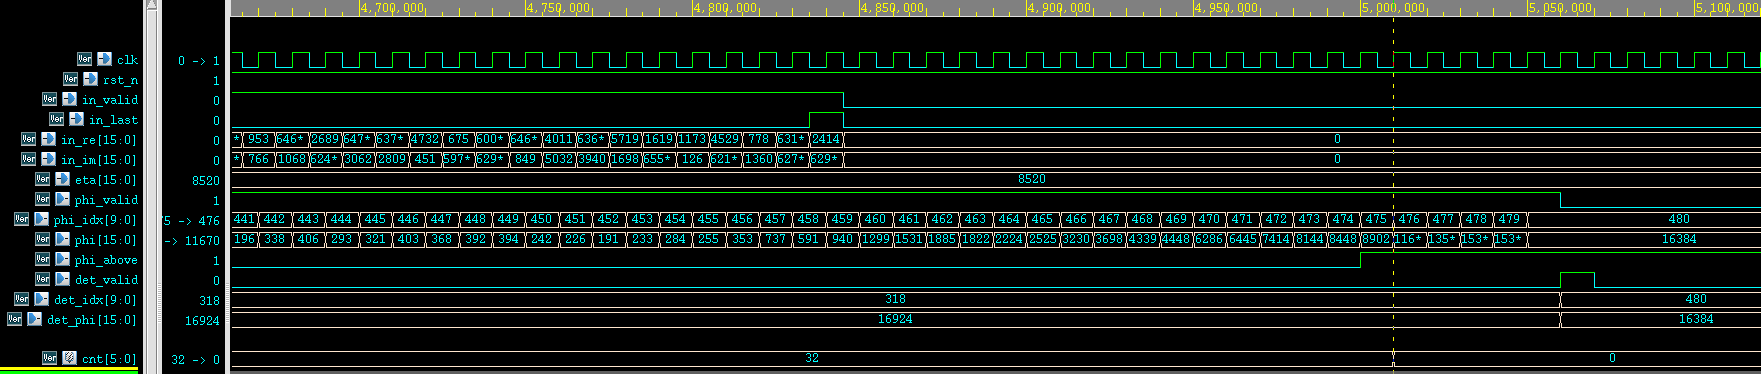
\includegraphics[width=\linewidth]{q3d_wave6.png}
    \caption{Behavioral Simulation: Last Boundary, $\hat m = 480$, Output by the Flush Rule}
    \label{fig:q3d_b3}
\end{figure}

In Figure~\ref{fig:q3d_b3}, \texttt{in\_last} marks the last input sample and \texttt{in\_valid} falls after it. The
search for the third lobe starts at $m = 475$ ($\Phi = 8902$). The last metric sample, $m = 480$ with $\Phi = 16384$
($= 1.0$), arrives 22 cycles after \texttt{in\_last}, and the flush rule outputs it one cycle later
(\texttt{det\_idx} = 480, \texttt{det\_phi} = 16384) instead of waiting for 32 more samples.

\subsection{Comparison with the Simulation}

Since the RTL output equals the bit-true model \texttt{sbd\_model.m} bit for bit, Figure~\ref{fig:q3d_cmp} draws the
hardware metric from that model on top of the floating-point $\Phi_{NM}$ of Q2.

\begin{table}[H]
\centering
\caption{Detected Boundaries: HDL versus MATLAB}
\setlength{\tabcolsep}{9pt}
\renewcommand{\arraystretch}{1.2}
\begin{tabular}{lccc}
\toprule
 & HDL & \makecell{MATLAB float,\\ same searcher} & \makecell{MATLAB, argmax\\ every symbol (Q2)} \\
\midrule
Noiseless & 165, 318, 480 & 165, 318, 480 & 160, 318, 480 \\
SNR 12 dB & 162, 320, 480 & 162, 320, 480 & 159, 162, 480 \\
\bottomrule
\end{tabular}
\end{table}

\begin{figure}[H]
    \centering
    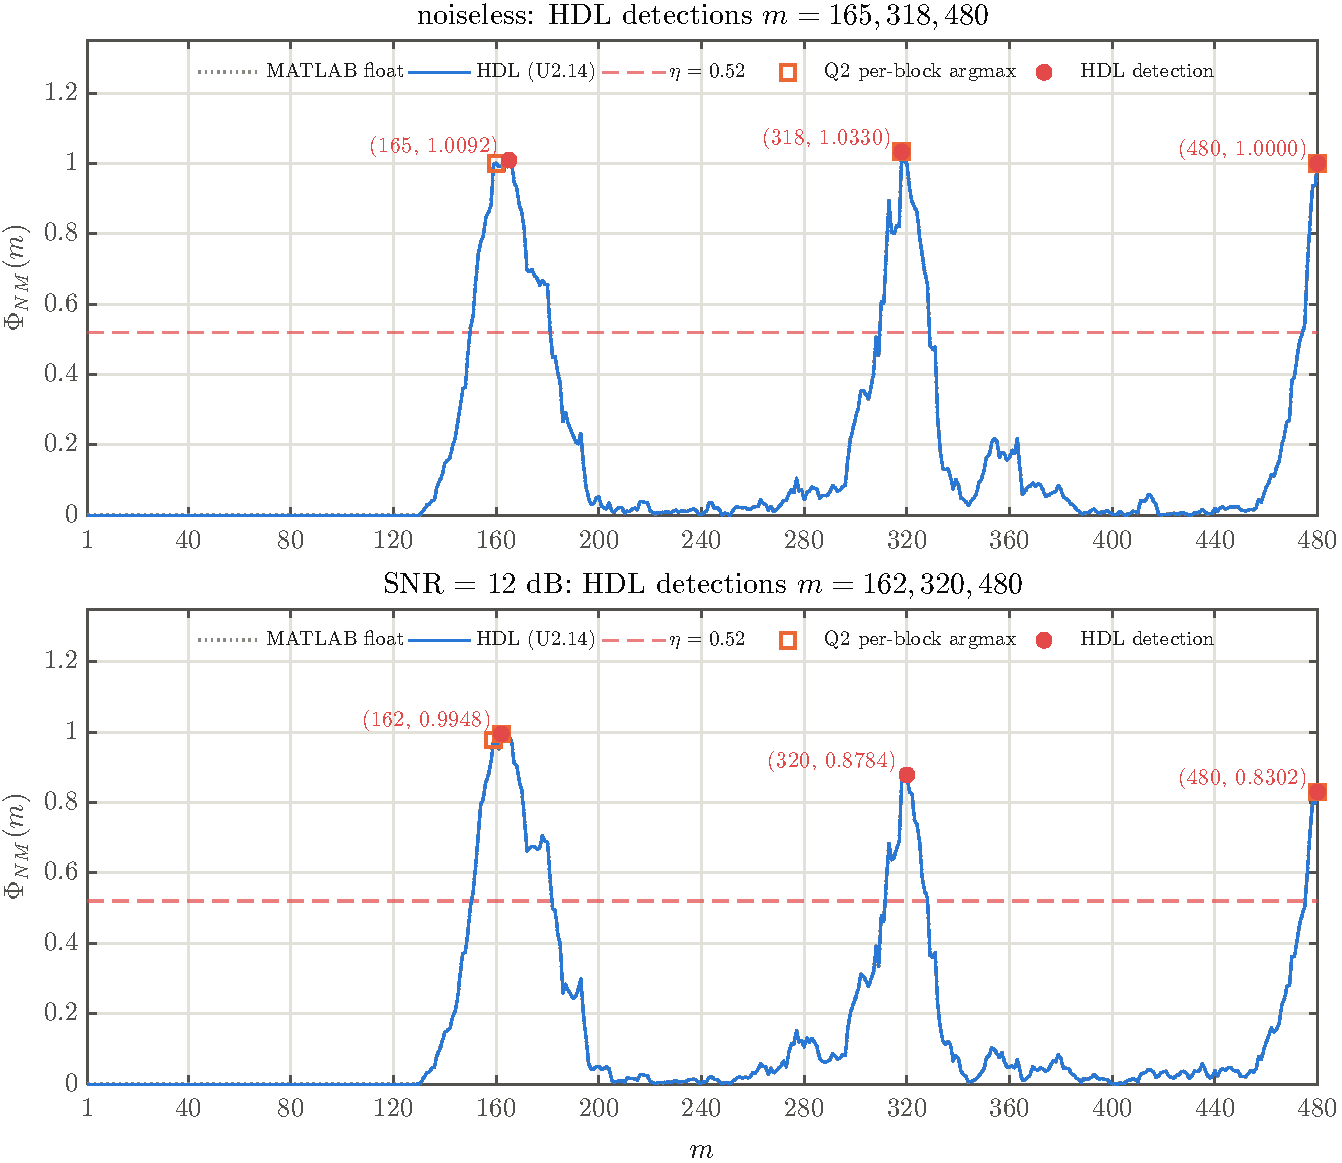
\includegraphics[width=0.86\linewidth]{q3d.pdf}
    \caption{Hardware Metric from the Bit-True Model, Equal to the RTL Output (blue), and Floating-Point $\Phi_{NM}$ (dotted), with the Hardware Detections (dots) and the Argmax of Every Symbol from Q2 (squares)}
    \label{fig:q3d_cmp}
\end{figure}

The two metric curves overlap; they differ by at most $9.3 \times 10^{-5}$. Running the same peak searcher on the
floating-point metric gives the same boundaries as the hardware, so quantization does not change any decision.

The differences from Q2 come from the decision rule. Q2 takes the maximum inside fixed 160-sample blocks, while the
hardware takes the maximum of each lobe above $\eta$. At 12\,dB this fixes symbol 2: the hardware finds 320, the
correct symbol end, where the block rule picked 162 from the previous lobe. In the noiseless case, though, the hardware
reports 165 for symbol 1 instead of 160, because $\Phi_{NM}(165) = 1.0092$ is 0.0092 larger than
$\Phi_{NM}(160) = 1$, the overshoot explained in Q2(c). The block rule could not pick 165 because 165 lies in the next block.

\newpage

% ─────────────────────────────────────────────
\chapter{AI Tool Disclosure}
\label{ch:ai}
% ─────────────────────────────────────────────
\question{Please disclose how you use AI tools and its version.}

I used \textbf{Claude Opus 5.5} to help with this homework in the following five parts:
\begin{enumerate}[label=(\arabic*)]
    \item Understanding the homework specification.
    \item Assisting with the MATLAB code.
    \item Assisting with the SystemVerilog RTL and testbench.
    \item Plotting the figures.
    \item Writing this \LaTeX{} report.
\end{enumerate}

\end{document}
